\documentclass{article}
\usepackage{a4wide}
\usepackage{listings}
\usepackage{url}
\usepackage[pdftex]{graphicx}
\usepackage{float}

\lstset{
basicstyle=\footnotesize,       % the size of the fonts that are used for the code
%breaklines=true,        % sets automatic line breaking
%breakatwhitespace=false,    % sets if automatic breaks should only happen at whitespace
%escapeinside={\%*}{*)},          % if you want to add a comment within your code
escapechar=\&,
}

\begin{document}

\title{Debugging AVR Raven with Contiki OS}
\author{Josef Lusticky}
\date{June 16, 2012}

\maketitle

This guide shows how to setup different tools for debugging.
Each of them has some pros and cons and each of them is preferred for other kind of development.

Debugging using the GNU Debugger with JTAG is easy to setup, works directly on the hardware
and usually needs only software available from a repository and no additional hardware setup.
But debugging using GDB might not be sufficient for all cases of development (such as the Timer/Counter modules).

A simulation of Contiki project with AVR Studio 4 can conveniently show all contents of memory
as well as registers - even each bit of them.
Values can be changed any time and this technique requires no hardware.
However, since AVR Studio~4 is only available for Windows OS,
a computer running Windows or virtual machine running Windows is required.
There is also no simple way of debugging a device using a network communication.

Debugging using serial output needs no extra software setup and is suitable
for debugging the whole system directly on the hardware.
Contiki is also well designed for this debugging technique.
The only major downside is a requirement of an additional hardware
for connection between the AVR Raven and the PC host.

%----------------------------------------------------------------------------

\section{GNU Debugger}
For debugging using the GNU Debugger we will use gdb-avr and avarice software -
an interface between GDB and AVR JTAG - avarice - {\url{http://avarice.sourceforge.net/}{.
Optionally we can also use DDD as a graphical frontend for debugging.

For debugging using GDB, we need already compiled project for AVR Raven.
\begin{lstlisting}
navigate to project directory we want to debug:
	&\textdollar& cd contiki/examples/hello-world
and compile it using make:
	&\textdollar& make TARGET=avr-raven
\end{lstlisting}
Avarice tool needs a hex file from our project.
If the hex file is not present in the project directory, the following command will extract it:
\begin{lstlisting}
extract a .hex file for flashing with avarice and other programmers:
	&\textdollar& make hello-world.hex
\end{lstlisting}

Next we lunch avarice which will also flash the project to hardware
through AVR Dragon and
create a port (1212) for connecting with the GDB debugger.
\begin{lstlisting}
	&\textdollar& avarice -g -j usb -P atmega1284p --erase --program --file hello-world.hex -B 1MHz :1212
\end{lstlisting}
After then we start the GDB debugger with our compiled binary file.
\begin{lstlisting}
the following will run gdb and drop us to its command line:
	&\textdollar& avr-gdb hello-wolrd.avr-raven
connect to 1212 port for communicating with the hardware, after then we can debug as usual:
	target remote :1212
run the program (we should set some brakepoints before):
	continue
\end{lstlisting}
If we want to use a DDD frontend, we start the DDD with avr-gdb debugger:
\begin{lstlisting}
	&\textdollar& ddd --debugger avr-gdb  hello-world.avr-raven
\end{lstlisting}
On the GDB Console connect to target using (if you can not see it, click View and then GDB Console):
\begin{lstlisting}
	(gdb) target remote :1212
\end{lstlisting}
Now we can select brakepoints and debug using continue as usual.

%----------------------------------------------------------------------------

\section{AVR Studio 4}
AVR Studio 4 is simulator of AVR platforms from Atmel.
Version 4 of AVR Studio is easy to get working with Contiki and provides everything needed for simulation.
Unfortunately AVR Studio is available only for Windows,
so we need a PC with Windows or Virtualbox with Windows installed on our Linux development PC.
The installation of Windows in Virtualbox is preferred because this way we can easily copy our compiled binaries
from the development Linux PC to Windows guest
without setting up build environment in Windows.
Of course we can use a separate computer with Windows for AVR Studio installation,
but in we will often copy files from development Linux PC.

\subsection{Installation}
Install Windows and the Guest addition in Windows if running under Virtualbox.
Set up shared folder (this needs the Guest additions) between your development host PC and virtual Windows PC, so you can copy files to Windows.
Install the AVR~Studio version~4.

Copy the complete Contiki source code with your compiled project from your development PC to
{\it{C:\textbackslash YOUR\_HOME\_FOLDER\_ON\_DEVELOPMENT\_PC\textbackslash}}
on Windows - e.g. your contiki source code is located at {\it{/home/josef/contiki}}
then you have to copy Contiki to directory \\
{\it{C:\textbackslash home\textbackslash josef\textbackslash contiki}}.
By other words - the root directory on your development PC remains root directory on Windows.

Similarly copy the avr header files usually from {\it{/usr/lib/avr/include}} to
{\it{C:\textbackslash usr\textbackslash lib\textbackslash avr\textbackslash include}}
and the avr-gcc header files usually from {\it{/usr/lib/gcc/avr/}}VERSION{\it{/include}} to \\
{\it{C:\textbackslash usr\textbackslash lib\textbackslash gcc\textbackslash avr\textbackslash VERSION\textbackslash include}}
where VERSION can be determined from {\it{avr-gcc -v}} command.
If the headers files are not to be found in this paths, {\it{avr-gcc -v }} command might help you to find them elsewhere.

If you will not stick to this paths on Windows,
you might be later asked by AVR Studio to locate these files and directories manually.

\subsection{Simulation}
Execute the AVR Studio 4.
From the Startup dialog select Open and open to your Contiki binary ELF file for AVR target
(it usually has {\it{.avr-raven}} name suffix).
If the Startup dialog is not shown, go to menu File and select Open File.
You will be asked where to save your newly created AVR Studio project (.aps file).
Choose anything you like ({\it{My Documents\textbackslash AVR}} fits good).
Now you will be asked to select the debug platform and the device.
Choose AVR Simulator and ATmega1284P for AVR Raven. (There seems to be a problem with the newer Simulator 2 with Timer/Counter 2 module).
You may be asked if you want to load EEPROM data - click OK.
Now you can simulate and debug you Contiki project in AVR Studio 4.
To select CPU frequency go to menu Debug and select AVR Simulator Options.
The Debug menu has all you need to step through the code. The I/O view shows current status of the hardware.

%----------------------------------------------------------------------------

\section{Serial Output}
Contiki configures USART~1 interface on AVR Raven for debugging in asynchronous operation
with the following parameters:
baud rate 57600, none parity, 1 stop bit, 8 data bits.
Contiki also automatically redirects stdout to this serial output, so every printf
writes to this interface.
In Contiki can be used PRINTF instead of printf, which outputs only if \#DEBUG is defined.
This configuration is defined and can be changed in
file {\it{contiki/platform/avr-raven/contiki-raven-main.c}},
{\it{initialize}} function - part commented with "Second rs232 port for debugging".

The USART~1 transmit output is Pin~3, Port~D (pins are numbered from zero in ATmega1284P datasheet),
$V_{CC}$ is Pin~7 on the bottom pin line on AVR Raven (these pin line is ATmega3290P interface and
pins are numbered from one in AVR Raven datasheet)
and ground is Pin~12 on the bottom line on AVR Raven (the rightmost pin).
This connection shows the figure bellow.
\begin{figure}[H]
  \centering
  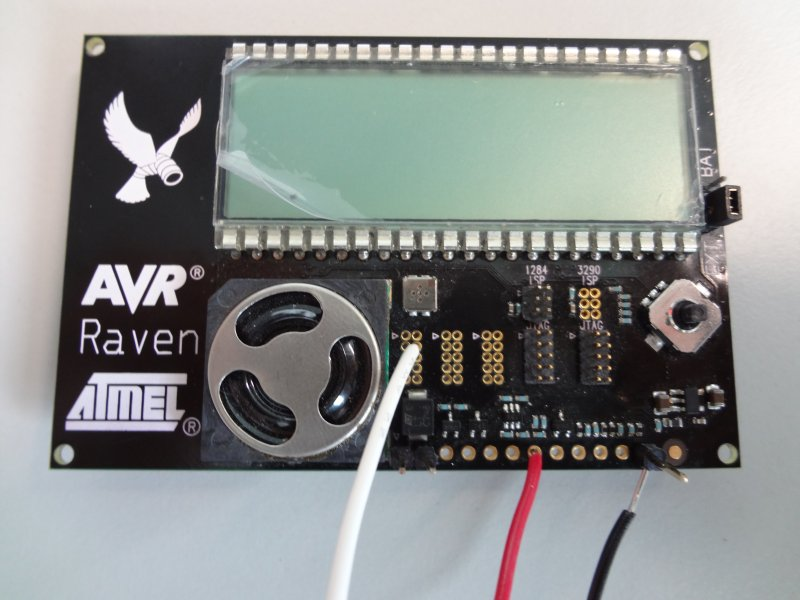
\includegraphics[width=12cm,keepaspectratio]{smallfig/DSC02579-small.jpeg}
  \caption{Serial output connection - white=rx, red=vcc, black=gnd}
\end{figure}

This output needs to be level shifted for RS232 using a MAX232 or similar chip,
because a desktop computer needs 5V and output from Raven is 3.3V.
Because many computers no longer have an RS232 serial port, a serial to USB converter might be needed.
Such a converter shows the following figure.
\begin{figure}[H]
  \centering
  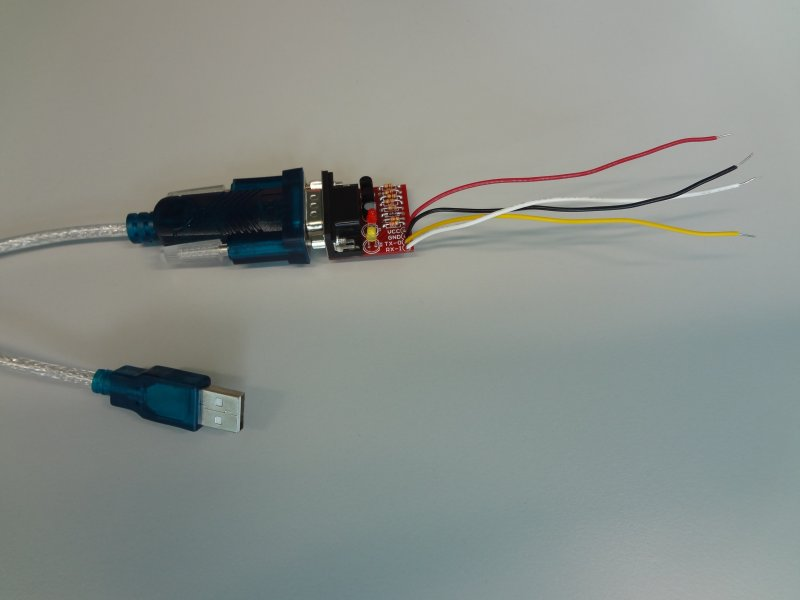
\includegraphics[width=9cm,keepaspectratio]{smallfig/DSC02577-small.jpeg}
  \caption{Serial to USB converter and level shifter}
\end{figure}

%----------------------------------------------------------------------------

\section{Other Tools}
AVR Raven device can be debugged using Cooja simulator, which is part of Contiki.
See {\url{https://www.sics.se/contiki/wiki/index.php/AVR_motes_in_COOJA}} for a tutorial on Contiki OS Wiki site.

There are plenty of other simulators and debugging techniques used, each of them suitable
different kind of debugging.
Among them HAPSIM simulator, SimAVR, Avrora or SimulAVR.

Contiki can also run on Unix-like systems. Use minimal-net or native target platform.
For Windows, target win32 can be used.
See {\url{https://www.sics.se/contiki/wiki/index.php/Setting_up_Wireshark_on_a_Loopback_Interface}}
for tutorial on Contiki OS Wiki site.
\end{document}
